\documentclass[conference]{IEEEtran}
\IEEEoverridecommandlockouts
% The preceding line is only needed to identify funding in the first footnote. If that is unneeded, please comment it out.
\usepackage{cite}
\usepackage{amsmath,amssymb,amsfonts}
\usepackage{algorithmic}
\usepackage{graphicx}
\usepackage{textcomp}
\usepackage{xcolor}
\usepackage[euler]{textgreek}
\def\BibTeX{{\rm B\kern-.05em{\sc i\kern-.025em b}\kern-.08em
    T\kern-.1667em\lower.7ex\hbox{E}\kern-.125emX}}
\begin{document}

\title{Creative Speech-to-Speech using MDRNN\\}

\author{\IEEEauthorblockN{1\textsuperscript{st} Vemund Sigmundson Schoyen}
\IEEEauthorblockA{\textit{ROBIN} \\
\textit{University of Oslo}\\
Oslo, Norway \\
vemund@live.com}
\and
\IEEEauthorblockN{2\textsuperscript{nd} Tony Nguyen}
\IEEEauthorblockA{\textit{ROBIN} \\
\textit{University of Oslo}\\
Oslo, Norway \\
hpnguyen@uio.no}
}

\maketitle

\begin{abstract}
Recent advances in recurrent neural networks have shown an unreasonable effectiveness of predictive sequence generation. Deep learning networks have shown capable in substituting complex analytic problems such as robotics control systems and image segmentation. In this paper, we try to substitute the intermediate steps in a speech-to-text and text-to-speech scheme for machine speech generation with a direct speech-to-speech model. 
\end{abstract}

\begin{IEEEkeywords}
RNN, LSTM, MDN, MFCC, speech-to-speech, deep learning
\end{IEEEkeywords}

\section{Introduction}
The use of recurrent neural networks (RNNs) has steadily grown due to their simplicity to model and their effectiveness in learning temporal data. RNNs can generate consecutive novel points in regards to an input sequence by remembering previously experienced sequences \cite{b6}. Some existing models even combine RNNs with a layer called mixture density layer (MDN), the combination is often abbreviated MDRNN, which recently has yielded excellent results. The Sketch-RNN model demonstrates the strength of MDRNN where a user draws a sketch in a continuous stroke in a 2D- plane, the Sketch-RNN will then attempt to draw the missing parts of the sketch after the user lifts the pen \cite{b7}. Another similar application developed by Alex Graves, where he uses MDRNN to effectively predict handwriting synthesis in a meaningful manner \cite{b6}. MDRNN has also been successfully applied in Robojam; an application used to predict appropriate touchscreen interaction locations in space and time for artificial music collaboration generation \cite{b5}. 

Recent advancement in GPU-development has led to increased computational resources. This had led to a lot of research into speech-synthesis, in particular, human speech generation, using neural networks. Recent work in this field relies heavily on text representations as an intermediate step for generating speech \cite{b11, b17}. Motivated to remove this intermediate step and to see if we can learn speech directly from raw audio data we look to similar research in this field. Although there is significantly less research in this area, there are a few noteworthy papers. 

State-of-the art methods include WaveNet and sampleRNN. WaveNet is a convolutional neural network model that has managed to greatly close the gap of making machines sound like humans \cite{b4}. sampleRNN is an RNN model that has achieved higher human evaluation ratings against their implementation of WaveNet on the speech synthesis task \cite{b16}. 

Babble-RNN created a speech-to-speech model using RNNs with the objective of imitating a speaker \cite{b1}. The results can be compared to a distorted baby-like speech signal. Although the babble-RNN does not create any meaningful novel speech, the results do show resemblance in pitch to the original speaker, and it seems as though the network learns natural pauses that occur in between words. 

The distortion is often a result of the encoding scheme of the speech sequence. This gives rise to an exploration for alternate encoding schemes which distorts the signal less, while maintaining the essence of the original speech.

Fredrik Bredmar uses direct speech-to-speech with LSTM-network with the objective of doing raw audio translation. Several tries resulted in only noise, while other attempts had initial periods of fair approximations to human-like speech, but ended in noise \cite{b2}.

John Glover uses raw musical audio, specifically piano and clarinet, to generate new audio using MDRNN. The results varied in quality, where the best result manages to imitate the keynote of the clarinet instrument relatively well \cite{b10}. 

In this paper we extend the babble-RNN model by substituting the last dense layer with a mixture density layer, making the overall model an MDRNN model. Furthermore, we propose an alternate encoding scheme than the Codec2 encoding used in Babble-RNN, namely the Mel-frequency cepstral coefficients (MFCCs).

\section{Background}

\subsection{Dataset}
We use a dataset of a single german speaker taken from Kaggle. The dataset contains about 3800 wav-files each a few seconds long. These audio files have a sample rate of 22050 samples per second. 
Although neither of the authors speak or understand German, this is not important as we expect the predicted sequences not to predict understandable words or sentences in German, but rather sounds that resemble the speaker.

\subsection{Long-short term memory}
RNNs are a variant of neural networks that try to learn temporal data but RNNs tend to forget when working with longer sequences \cite{b6, b8}. Several approaches have been proposed to solve this problem, where arguably the most popularly applied model is the LSTM model. 

Long short-term memory (LSTM) is an RNN architecture designed to improve its property of storing and accessing information than its RNNs counterpart by implementing a memory cell called LSTM-cell \cite{b13}. Advantages of such capability are generating sequences while reminiscing previous inputs over longer durations than RNNs. Hence, LSTM-networks proves more efficient for future predictions than for standard RNNs \cite{b6}.

\subsection{Mixture density networks}
The idea of mixture density networks can be explained by the problems of non-mixture density networks. General neural networks that use a dense layer as its last layer can, based on an input, predict its corresponding output value. The problem arises when identical or similar inputs map to different outputs. Instead of learning the direct map from inputs to outputs, you instead learn the map from inputs to a mixture of distribution parameters \cite{b3}. This can be viewed as logically equivalent to a softmax function, except for the continuous case, whereas softmax is for the discrete case.

Martin's implementation of a mixture density layer assumes a collection of scaled Gaussian distributions, which is often called a Gaussian mixture model (GMM). The outputs from the GMM consists of means \boldmath$\mu$, standard deviations $\sigma$ and scalings $\pi$ describing the Gaussian mixture distribution. \unboldmath

The loss function used can achieve arbitrarily low values. In general, the smaller the loss, the better we fit our data. Thus, high negative values is often an indication of a good fit \cite{b5}.

We used the implementation of the mixture density layer with corresponding loss function compatible with keras developed by Charles Martin which can be found here:
https://github.com/cpmpercussion/keras-mdn-layer

\subsection{Mel-frequency cepstral coefficients}
The MFCC transform is a speech compression scheme using the Mel scale to include the most important frequencies describing pitches in human speech.

The MFCC transform consists of several steps. Begin by performing a Fourier transform on a part of the temporal input signal using a windowing function (we use the default from librosa, i.e. Hann). This part is now described in full by its frequency spectrum. Next, we look at the squared magnitude of the frequency spectrum, called the power spectrum. 

Now we apply the Mel-scale to our power spectrum. The Mel-scale is a perceptual scale, meaning that it has been created based on humans listening to speech signals and deciding the most important pitches. In practice, this is done using partially overlapping windows for the most important frequencies in the power spectrum. Here we can choose the number of frequencies we want, higher amount gives less compression but retains more of the original signal.

Then perform a logarithmic transform on the Mel-scaled power spectrum. Lastly, perform a discrete cosine transform (DCT) on the log-transformed Mel-frequencies as if this itself were a signal. The resulting amplitudes of this spectrum are the MFCCs. \cite{b14, b15}

Creating a pseudo-formal approach for conceptual clarity. Given a signal:
\[\textbf{t} = (t_0, t_1, ..., t_i, ...,  t_N) \]
where each element t represents an amplitude of a sampled signal at time i. Then a MFCC transform will yield:

\[MFCC(\textbf{t}) = (\textbf{MFCCs}_0^T, \textbf{MFCCs}_1^T, ..., \textbf{MFCCs}_M^T)\]

The transformed signal is now a two-dimensional matrix with MFCCs in one direction and temporal information in the other direction. This can be viewed as a spectrogram. Figure \ref{fig1} displays our best result as a spectrogram made by using FFmpeg. Although this method is not directly related to the MFCC transform, it conveys the general idea of how the MFCC spectrogram looks.

\begin{figure}[ht] 
  \centering %midtstilt figur
  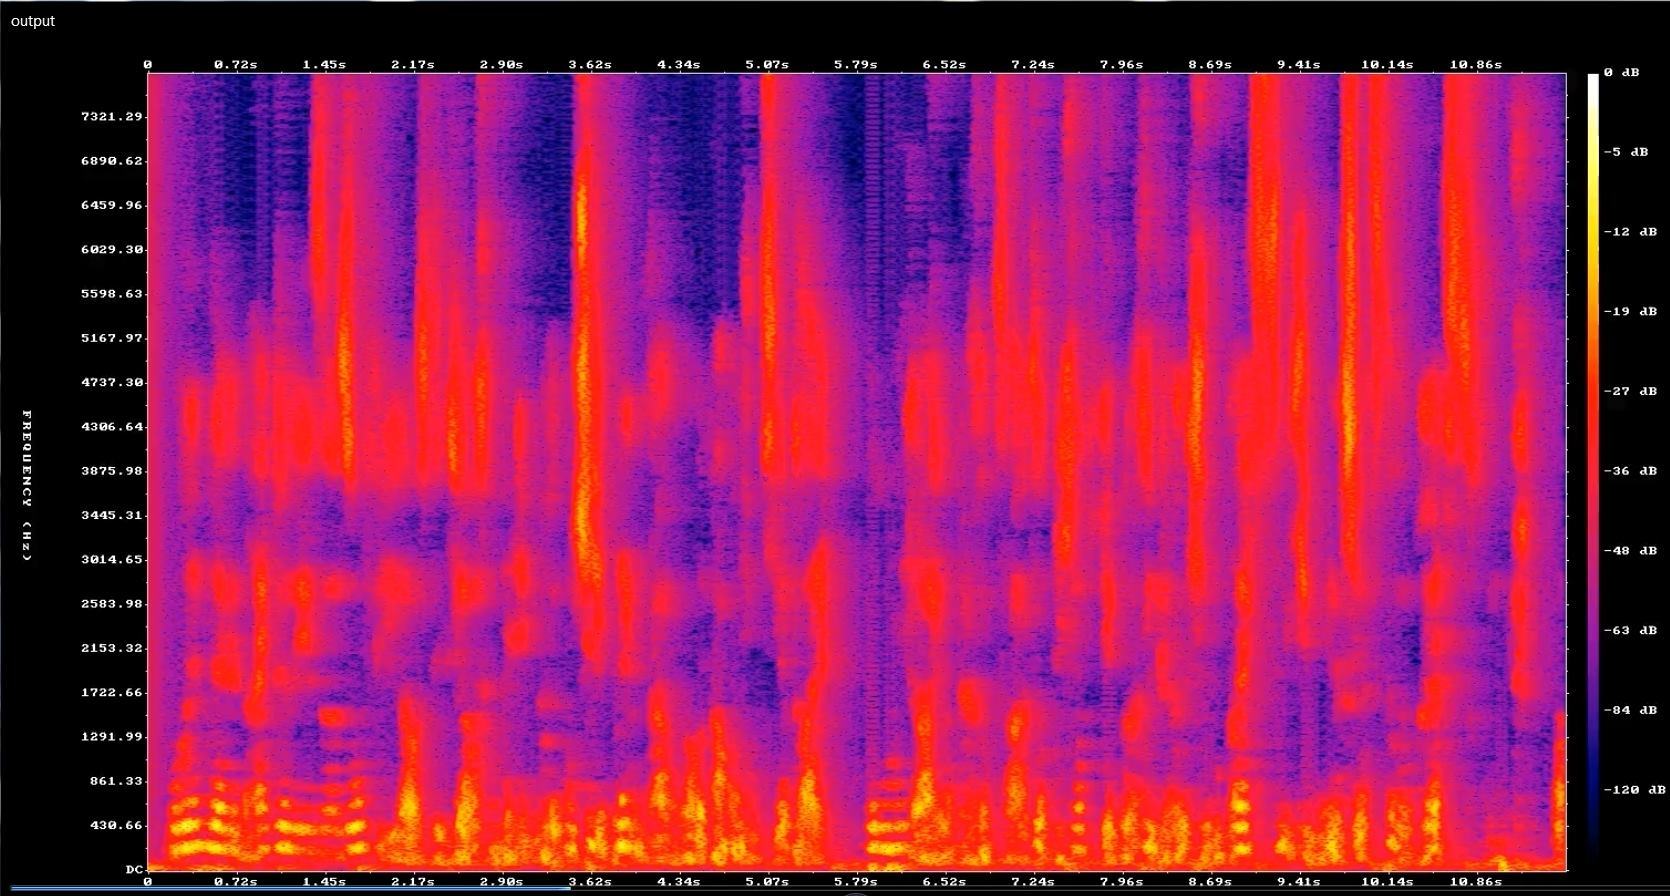
\includegraphics[width=0.39\textwidth]{./best/spectrogram.jpg} 
  \caption{Spectrogram of the time-distributed simple model using FFmpeg. Showing the frequencies in the y-direction and time in the x-direction}
  \label{fig1} 
\end{figure}

In our implementation, we use the built-in function from librosa which automatically encodes an audio signal to MFCCs. 

\subsection{Normalization/denormalization}
We implement three different normalization versions with corresponding denormalization. The first version normalizes the data to the interval: [0, 1]. The second approach normalizes between [-1, 1] since the LSTM layers use the tanh activation function. Both of the above methods rely on the maximum and minimum of the data for denormalization; thus this is stored. The last approach standard normal distributes the data, i.e., N(0, 1), which relies on the mean and standard deviation of the data for denormalization, thus this is stored.

We implement these normalization and denormalization versions such that we can choose which normalization we want before any training run of the network. Now we have three normalization versions as hyperparameters.

\subsection{Creating trainable data}
There are several ways to structure our training data. To make it clear how we structure our data, we shall introduce some notation first. We shall denote a training data element 
\[ (\textbf{x}^i,\textbf{y}^i)\] 
where \textbf{x} and \textbf{y} represents  input and target sequence pair \textit{i} respectively. 

We shall call the training data structure 
\[ \textbf{x}^i = (\textbf{x}_0^i, \textbf{x}_1^i, ..., \textbf{x}_{n-1}^i), \] 
\[\textbf{y}^i = \textbf{x}_n^i\] 
where the next training pair is time-shifted by one element, i.e:
\[ \textbf{x}^{i+1} = (\textbf{x}_0^{i+1}, \textbf{x}_1^{i+1}, ..., \textbf{x}_{n-1}^{i+1}) = (\textbf{x}_1^i, \textbf{x}_2^i, ..., \textbf{x}_n^i),\]
\[ \textbf{y}^{i+1} = \textbf{x}_n^{i+1} = \textbf{x}_{n+1}^i\] 
the \textit{simple model}. 

Note here that an element 
\[\textbf{x}_{j}^i\] 
correspond to an m-dimensional vector. In our case, this corresponds implicitly to our MFCCs. Although explicitly (in the case of using MDs as the final layer) this correspond to our mixture distribution parameters which we use to sample our MFCCs.

A similar approach to the simple model can be used in the case of a time-distributed network. This means that instead of predicting only the next novel point based on the entire input sequence, we instead force the network to predict each next point in the sequence, including the novel point. We shall call this model \textit{time-distributed simple model}.

From here it is clear that our input and target data highly overlapping, i.e the target data is contained in the input data at consecutive time steps. This leads to the idea of trying to reduce the overlapping of input and training data, at least to some degree. Lets describe this formally:

\[ \textbf{x}^i = (\textbf{x}_0^i, \textbf{x}_1^i, ..., \textbf{x}_{n-1}^i), \] 
\[\textbf{y}^i = (\textbf{x}_1^i, \textbf{x}_2^i, ..., \textbf{x}_n^i)\] 
where the next training pair is time-shifted by k elements, i.e:
\[ \textbf{x}^{i+1} = (\textbf{x}_0^{i+1}, \textbf{x}_1^{i+1}, ..., \textbf{x}_{n-1}^{i+1}) = (\textbf{x}_k^i, \textbf{x}_{k+1}^i, ..., \textbf{x}_{k+n}^i)\]
\[ \textbf{y}^{i+1} = (\textbf{x}_1^{i+1}, \textbf{x}_2^{i+1}, ..., \textbf{x}_n^{i+1}) =(\textbf{x}_{k+1}^i, \textbf{x}_{k+2}^i, ..., \textbf{x}_{k+n+1}^i)\]
We call this model \textit{time-distributed k-shifted model}. Notice that this can naturally be extended for the simple model as well, without explicitly noting it, we call this approach \textit{k-shifted model}.

Choosing k=1 results in the simple models, while choosing k=n+1 yields a mutually exclusive training set.

We implement a general approach to these ideas and include k as a hyperparameter.

\section{System design/Model}
The librosa library MFCC transform automatically creates our desired temporal MFCC matrix from an arbitrarily long one-dimensional signal. Thus we start by concatenating as many wav-files as we want to train on. The memory requirement strongly depends on the choice of training data model. Note that the simple models require a lot of duplication of data to be stored in memory, while a k-shifted model can hold more unique data in memory since there is less overlap in the training data. 

Before we start creating input and target data from our temporal MFCC matrix we normalize it by one of the above-mentioned normalization schemes.

We train for a number of specified epochs which we choose as a hyperparameter. However, by saving our model we can always continue training our model for an extended period if the chosen hyper-parameters seems to produce reasonable results but requires more training. An indication of how well we are generalizing can be seen from the validation loss after each epoch of training.

After we are satisfied with our loss, we can start to generate a new speech signal. We begin by predicting a single novel point by feeding a start sequence into our trained model which generates a vector of parameters to a mixture density distribution. Sampling this distribution yields a novel point corresponding to a vector of MFCCs. This novel point can then be appended to the input sequence and then removing the first point in the input sequence to retain the original sequence length. Feeding this new sequence into our model again predicts another novel point. Following this approach, we can generate an arbitrarily long novel sequence. 

Lastly, we need to denormalize our new sequence based on the stored normalization parameters followed by an inverse MFCC transform. The results are a predicted one-dimensional wav-signal which we can listen to.

The following algorithmic steps can explain the above description:
\begin{enumerate}
    \item Concatenate wav-files
    \item Encode concatenated sequence (MFCCs)
    \item Normalize data
    \item Create trainable data set 
    \item Train MDRNN model for a number of epochs
    \item Repeat 
         \begin{enumerate}
        \item Predict distribution parameters based on input sequence
        \item Sample novel point (MFCCs) from distribution
        \item Remove first element from input sequence, add predicted novel point to the end
    \end{enumerate}
    \item Denormalize predicted sequence
    \item Decode sequence using inverse MFCC
\end{enumerate}

\section{Deciding network topology and tuning hyper parameters}
There are a lot of hyperparameters in our model. During training, we discovered a few models, i.e., choice of hyperparameters that generated relatively qualitatively good results. We shall present the hyper parameters of the best performing model. Our model uses the time-distributed simple model which we abbreviate TDSM.

\begin{table}[htbp]
\caption{Table of hyper parameters}
\begin{center}
\begin{tabular}{|c|c|}
\hline
\textbf{Hyper parameters} & \textbf{\textit{TDSM}} \\
\hline
Normalization method & N(0, 1) \\
\hline
k (time-distributed k-shift)& 1 \\
\hline
Number of files & 10 \\
\hline
Number of MFCC & 35 \\
\hline
Input length & 101 \\
\hline
Number of epochs & 100 \\
\hline
LSTM topology & 3-stacked, 200 units \\
\hline
Number of mixtures & 5 \\
\hline
Batch size & 64 \\
\hline
validation split & 0.15 \\
\hline
Number of predictions & 400 \\
\hline
Optimizer & Nadam \\
\hline
\end{tabular}
\label{tab1}
\end{center}
\end{table}

\section{Results}
Our most important measurement is a qualitative one. Meaning, the experience of listening to the generated audio. Otherwise, we performed some documentation of the loss during training, statistics of the MDN output and the actual generated sound wave. These can be seen from the figures displayed below. 

The prediction statistics from figure \ref{fig2} displays the predicted average, standard deviation, maximum and minimum of means against the standard deviations \boldmath$\sigma$, means $\mu$ scalings $\pi$ of the trained network. The essential trait here is that the variables mentioned above behave nicely. Meaning we do not want unusual spikes or deviations from the early predictions. Since our network is eventually predicting on predictions this could result in compounding errors which could make later predictions have unwanted behavior as in Bredmars case \cite{b2}. \unboldmath

From figure \ref{fig2} we see the trend that we want in our predictions. Especially that the longer we get into our predictions they still behave similarly as the early predictions.

\begin{figure}[ht] 
  \centering %midtstilt figur
  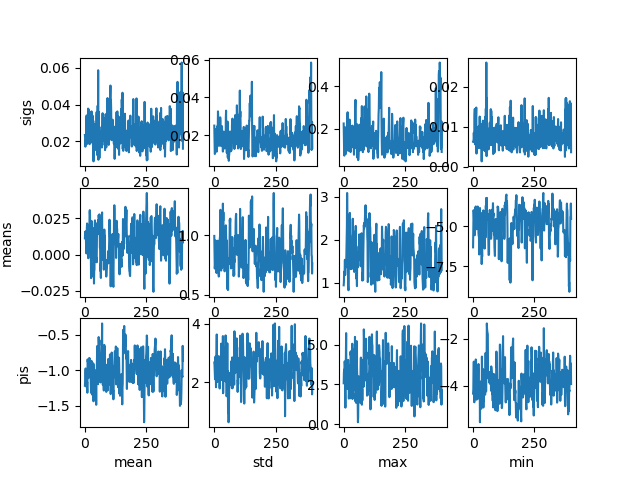
\includegraphics[width=0.39\textwidth]{./best/BEST2_stats.png} 
  \caption{Prediction statistics of time-distributed simple model. The x-axis' for each of the plots are the MDN parameter predictions, here 400}
  \label{fig2} 
\end{figure}

The training statistics from figure \ref{fig3} shows us how the statistics mentioned above evolve during our training. They are sampled after each epoch of the training period. The most important figures to pay attention to here is the standard deviations \boldmath$\sigma$ row. This shows us how confident the network is getting during training. The lower standard deviations we get, the more confident the network becomes. We especially want a low maximum, since this restricts the other statistics of the standard deviations $\sigma$. \unboldmath

From figure \ref{fig3} we see the trends in the standard deviations \boldmath$\sigma$ that we want. In particular look at how the maximum of the standard deviations $\sigma$ is decreasing towards zero. \unboldmath

\begin{figure}[ht] 
  \centering %midtstilt figur
  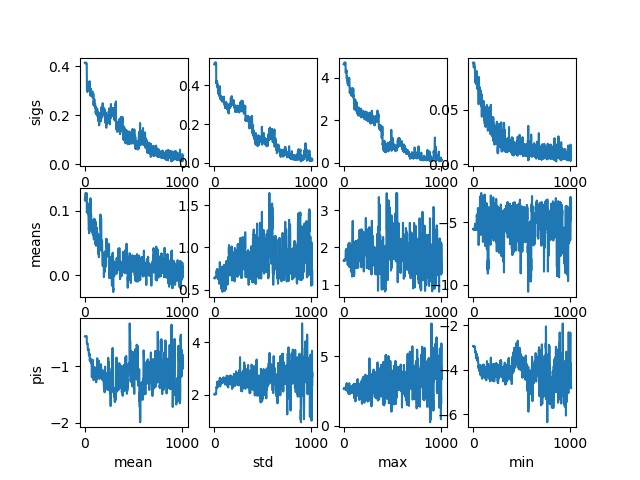
\includegraphics[width=0.39\textwidth]{./best/BEST2_train_stats.png} 
  \caption{Training statistics of time-distributed simple model. The x-axis is the 10*MDN parameter predictions per epoch}
  \label{fig3} 
\end{figure}

Figure \ref{fig4} shows the training and validation loss over the training period. We see a good trend in the training loss, but a bad validation loss. In general, this would be a strong indication of overfitting. One could argue that having a poor validation loss would yield poor results when performing predictions on unseen input, which is what we will eventually input to our network when performing consecutive predictions on predicted sequences. However, since we value a qualitative analysis higher than our statistics, we have experienced poor results when stopping training early, i.e., when the validation loss is still low. 

\begin{figure}[ht] 
  \centering %midtstilt figur
  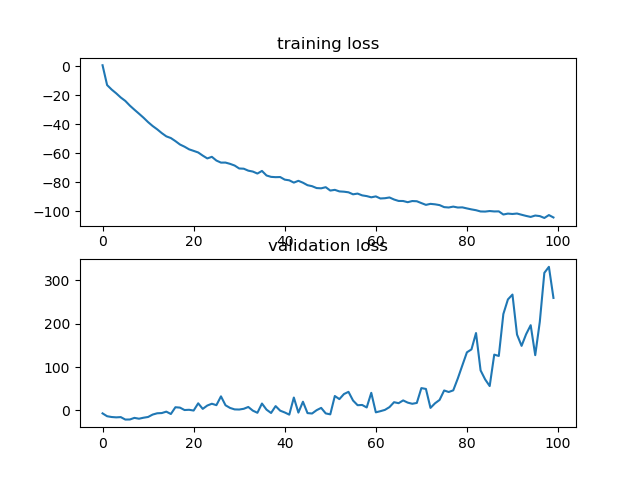
\includegraphics[width=0.39\textwidth]{./best/BEST2_loss.png} 
  \caption{Loss and validation loss of time-distributed simple model over the 100 epochs of training}
  \label{fig4} 
\end{figure}

Figure \ref{fig5} shows the actual generated sound waves. The first two seconds are from the original signal after an MFCC transform and inverse transform. The following seconds are the network predicted values which looks similar to the first few seconds. This is a good indication.

\begin{figure}[ht] 
  \centering %midtstilt figur
  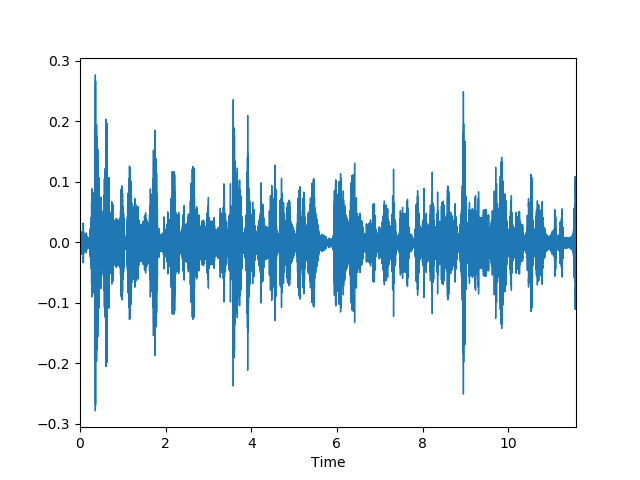
\includegraphics[width=0.39\textwidth]{./best/BEST2.png} 
  \caption{Sound wave of time-distributed simple model}
  \label{fig5} 
\end{figure}

We use the minimum-mean-square-error short-time spectral amplitude estimator (MMSE-STSA) algorithm on the outputted sound wave to make the overall signal clearer by reducing some of the noise \cite{b9}.

\section{Discussion}
When listening to the predicted sequence, we hear that it imitates the original signal very well, keeping the same tone as the speaker. There are even instances that resemble actual words. As the authors do not speak German, we can not deduce if this is the case. Furthermore, the signal does not seem to be repeating itself, so the new sequence is a creative one!

During the development of our model, we experienced difficulties when trying to get stable predictions, which might be due to several factors. If the standard deviations \boldmath$\sigma$ is high, we can get relatively large deviations from the normal MFCC value range. Combining this with the inverse MFCC transform including an exponential conversion which makes small changes in MFCC predictions yield large values for the reconstructed, partially predicted signal. These large values present themselves as spikes in our reconstructed signal which wash out all other parts of the signal making it very tough to understand exactly how this happened. This makes the choice of hyperparameters extra important to get reasonable results. \unboldmath

\section{Conclusions}
We are very impressed by the results obtained by our model. By listening to babble-rnn and comparing it to our best results, we conclude that including a mixture density network does improve predictive imitations of a single speaker. 

\section{Future work}
As the choice of hyperparameters dramatically influences the quality of the network predictions we advocate doing more thorough testing of these. This could potentially produce much better results than we discovered during our trials.

It could also be interesting to see how our implementation of MDRNN would perform using codec2, as in babble-rnn.

\section*{Acknowledgment}
We want to give a special thanks to Charles Martin for his numerous contributions and helpful feedback during the entirety of this project.

\begin{thebibliography}{00}
\bibitem{b1} Phil Ayres (25 May 2017). Babble-rnn: Generating speech from speech with LSTM networks' [Blog post]. Retrieved from http://babble-rnn.consected.com/docs/babble-rnn-generating-speech-from-speech-post.html

\bibitem{b2} Fredrik Bredmar, ``Speech-to-speech translation using deep learning". Univeristy of Gothenburg, 2017.

\bibitem{b3} C. Bishop. ``Mixture density networks". Technical report, 1994.

\bibitem{b4} Aäron van den Oord, Sander Dieleman, Heiga Zen, Karen Simonyan, Oriol Vinyals, Alex Graves, Nal Kalchbrenner, Andrew Senior, Koray Kavukcuoglu ``Wavenet: a generative model for raw audio'' Google, London, UK, 2016.

\bibitem{b5} Charles Martin, Jim torresen, ``'Robojam, Musical Mixture density for Collaborative Touchscreen Interaction'',
	University Of Oslo, November 30, 2017

\bibitem{b6} Alex Graves, ``Generating sequences with recurrent neural networks'' University of Toronto, 5. jun. 2014.

\bibitem{b7} David Ha, Douglas Eck, ``A Neural Representation of Sketch Drawings'' 19. may. 2017.

\bibitem{b8} S. Hochreiter, Y. Bengio, P. Frasconi, and J. Schmidhuber. ``Gradient Flow in Recurrent Nets: the Difficulty of Learning Long-term Dependencies." In S. C. Kremer and J. F. Kolen, editors, A Field Guide to Dynamical Recurrent Neural Networks. 2001.

\bibitem{b9} Yariv Ephraim, David Malah , ``Speech Enhancement Using a Minimum Mean-square Error Short-time Spectral Amplitude Estimator", VOL. ASSP-32, NO.6, December 1984

\bibitem{b10} John Glover (16 December 2015). Generating sound with recurrent neural networks [Blog post]. Retrieved from http://www.johnglover.net/blog/generating-sound-with-rnns.html

\bibitem{b11} Yuxuan Wang, RJ Skerry-Ryan et al. ``Tacotron: Towards End-to-End Speech Synthesis", Google Inc, 6. April 2017  

\bibitem{b12} M. Schuster, ``Better generative models for sequential data problems", Neural Information Processing Systems, 1999

\bibitem{b13} S. Hochreiter, J Schmidhuber ``Long Short-term Memory, Neural Computation", 1997

\bibitem{b14} Shikha Gupta, Jafreezal Jaafar et al. ``Feature Extraction Using MFCC", An international Journal(SIPIJ) Vol.4, No.4, August 2013

\bibitem{b15} Parwinder Pal Singh, Pushpa Rani, ``An Approach to Extract Feature using MFCC", Journal of Engineering(IOSRJEN) Vol. 04, Issue 08, August 2014

\bibitem{b16} Soroush Mehri, Kundan Kumar et al ``SampleRNN: An Unconditional End-to-End Neural Audio Generation Model", ICLR 2017, 11 February 2017

\bibitem{b17} Ye Jia, Yu Zhang et al., ``Transfer Learning from speaker Verification to Multispeaker Text-To-Speech Synthesis", 5. November 2018
\end{thebibliography}


\end{document}
